\paragraph{Predeclared conditional eligibility.}
joint-improvement: 77 eligible. The selected lower-median example appears in Fig.~\ref{fig:final-qualitative-03}.
geometry-loss: 191 eligible. The selected lower-median example appears in Fig.~\ref{fig:final-qualitative-04}.
appearance-loss: 153 eligible. The selected lower-median example appears in Fig.~\ref{fig:final-qualitative-05}.
Overlapping conditions share one panel. The first outcome-blind panel stays in the Main text even when it also satisfies a conditional category; it is referenced here rather than duplicated.
\begin{figure*}[!t]
\centering
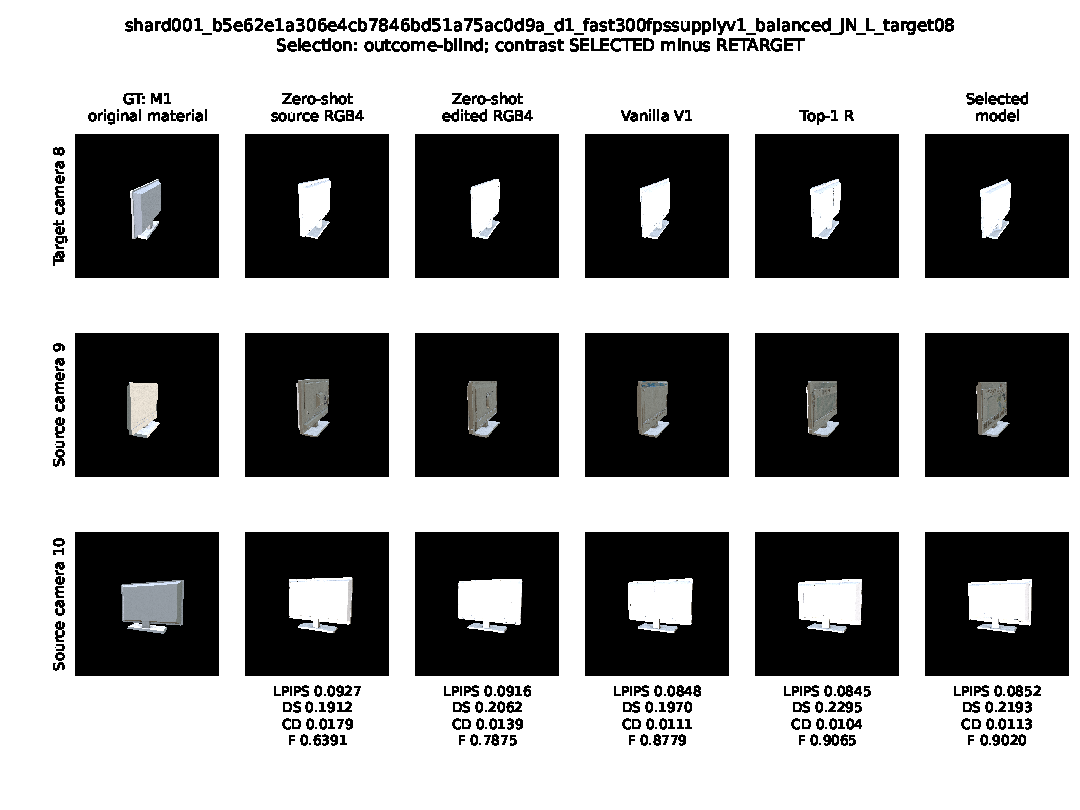
\includegraphics[width=\textwidth]{final-results/figures/example-02.pdf}
\caption{Actual scored frozen TEST example. Rows are target8/source9/source10; columns are the common original-material M1 reference and every frozen model. Selection: outcome-blind. Full-frame panels use the scored archive and official uint8 conversion, without model-specific crop, alignment or rerender. Source annotations use cameras9/10. Conditional categories illustrate their stated conditions and do not estimate population success rates.}
\label{fig:final-qualitative-02}
\end{figure*}
\begin{figure*}[!t]
\centering
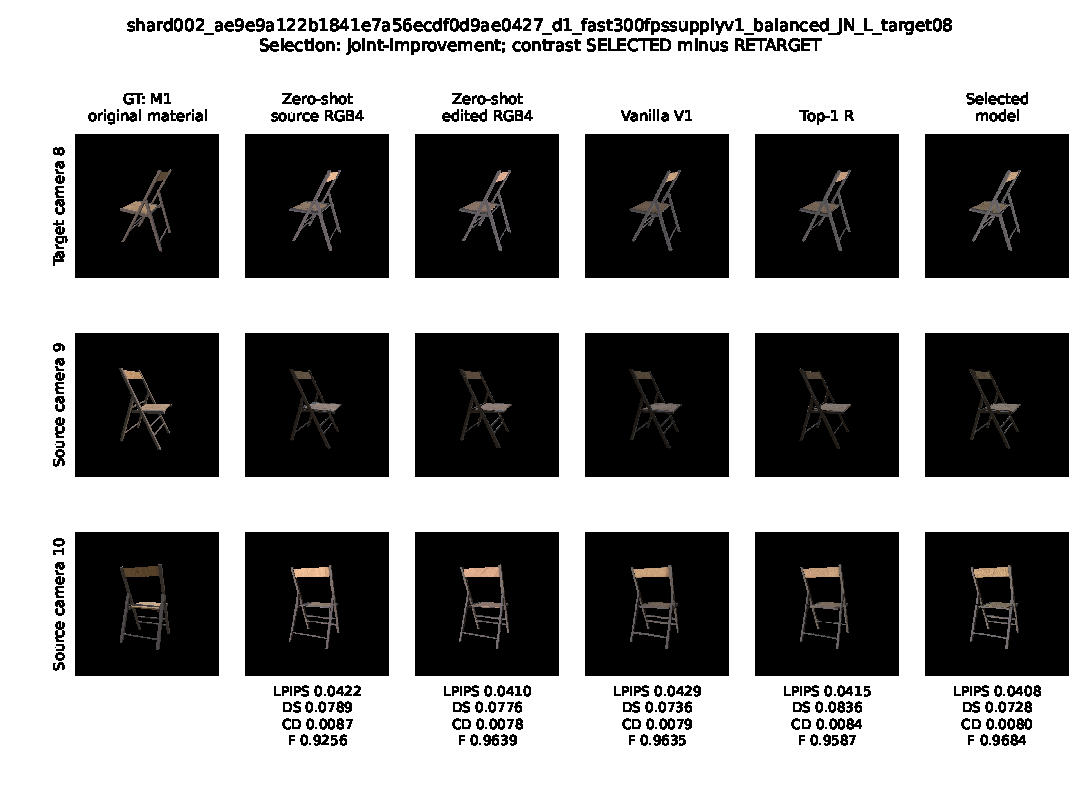
\includegraphics[width=\textwidth]{final-results/figures/example-03.pdf}
\caption{Actual scored frozen TEST example. Rows are target8/source9/source10; columns are the common original-material M1 reference and every frozen model. Selection: joint-improvement. Full-frame panels use the scored archive and official uint8 conversion, without model-specific crop, alignment or rerender. Source annotations use cameras9/10. Conditional categories illustrate their stated conditions and do not estimate population success rates.}
\label{fig:final-qualitative-03}
\end{figure*}
\begin{figure*}[!t]
\centering
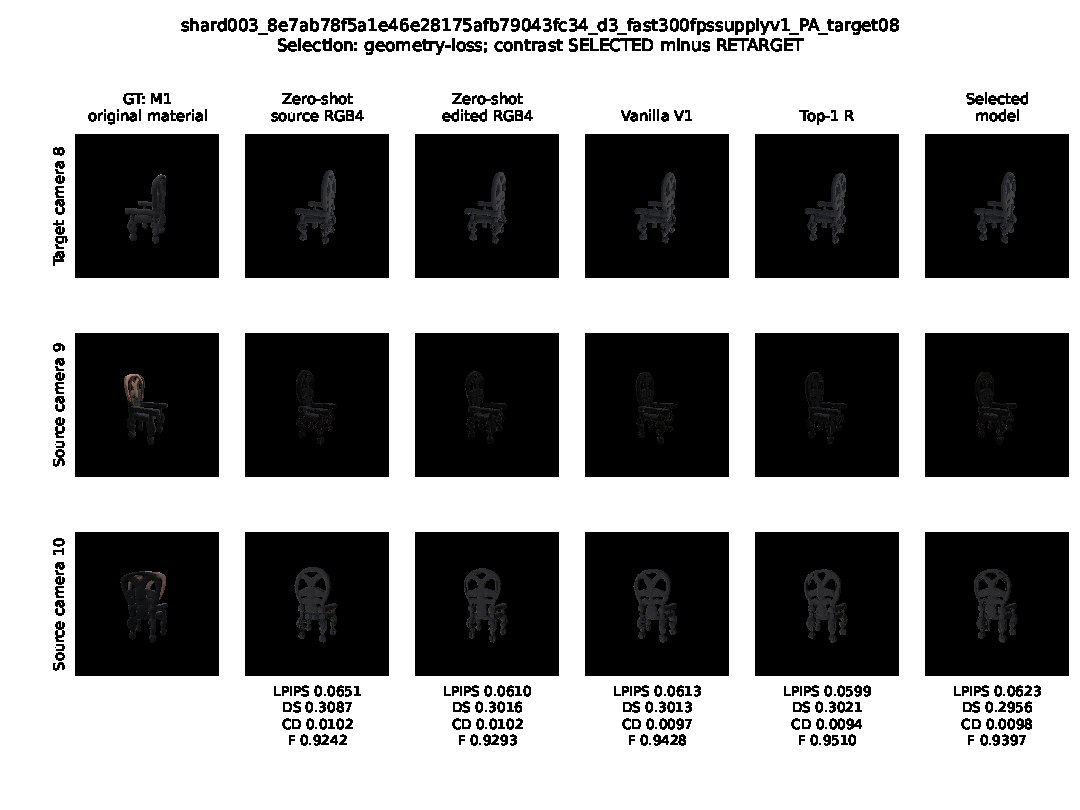
\includegraphics[width=\textwidth]{final-results/figures/example-04.pdf}
\caption{Actual scored frozen TEST example. Rows are target8/source9/source10; columns are the common original-material M1 reference and every frozen model. Selection: geometry-loss. Full-frame panels use the scored archive and official uint8 conversion, without model-specific crop, alignment or rerender. Source annotations use cameras9/10. Conditional categories illustrate their stated conditions and do not estimate population success rates.}
\label{fig:final-qualitative-04}
\end{figure*}
\begin{figure*}[!t]
\centering
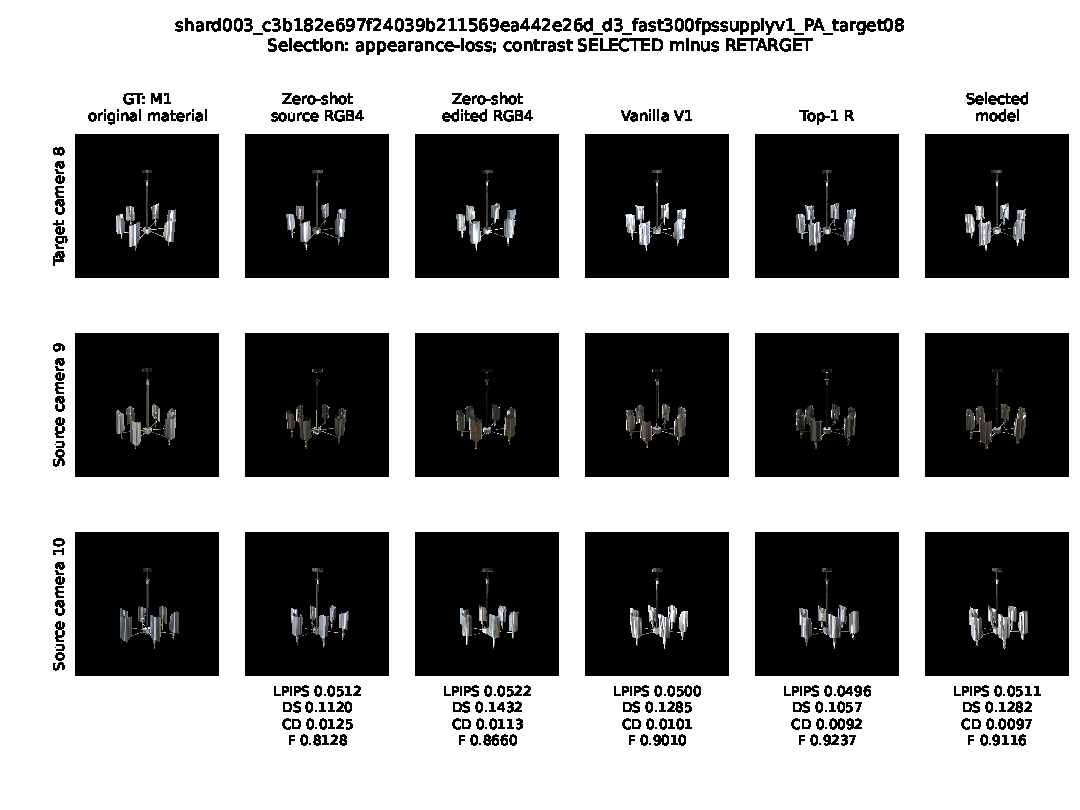
\includegraphics[width=\textwidth]{final-results/figures/example-05.pdf}
\caption{Actual scored frozen TEST example. Rows are target8/source9/source10; columns are the common original-material M1 reference and every frozen model. Selection: appearance-loss. Full-frame panels use the scored archive and official uint8 conversion, without model-specific crop, alignment or rerender. Source annotations use cameras9/10. Conditional categories illustrate their stated conditions and do not estimate population success rates.}
\label{fig:final-qualitative-05}
\end{figure*}
